\section{Сбор новостей} \label{sec:collecting}
Сбор актуальных новостей является важной задачей в разрабатываемой системе, потому что качество и актуальность собранной информации влияет на выделение сюжетов, что, в свою очередь, виляет на ранжирование источников.

С данной задачей связано большое количество проблем: огромное число новостных источников, ограничительная пропускная способность каналов, зашумлённость страниц второстепенной информацией и так далее.

\subsection{Новостные ленты}
Большинство новостных источников, включая новостные сайты и популярные группы в социальных сетях, предоставляют rss- и atom- ленты~--- небольшие xml-документы, в которых описываются последние новости и ссылки на них. Такие ленты стараются поддерживать актуальными, поскольку они используются многими новостными агрегаторами, которые активно используются пользователями.

Важно отметить, что в самих лентах не хранится непосредственно текст новостей, а лишь ссылки на html-страницы, расположенные на сайте источников, поэтому после получения ленты необходимо выгружать страницы с сайта источника.

\subsection{Фильтрация посещённых страниц}
Один источник может предоставлять несколько лент, например по ленте на категорию или тематику. Поэтому одна и та же новость может быть получена из нескольких лент, что будет создавать дополнительную нагрузку на систему. Поэтому имеет смысл отбрасывать уже посещённые новостные страницы. Очевидное на первый взгляд решение проблемы~--- использование ассоциативных массивов~--- довольно требовательно к памяти, поэтому имеет смысл рассмотреть использование вероятностных фильтров. Наиболее популярным фильтром подобного рода является фильтр Блума.

\subsubsection{Фильтр Блума} \label{sssec:bloom-filter}
Фильтр Блума~--- вероятностная структура данных, позволяющая компактно хранить множество элементов и проверять принадлежность заданного элемента к множеству. При этом существует вероятность получить ложноположительный результат, то есть ситуацию, когда элемента в множестве нет, но фильтр сообщает, что элемент есть.

Фильтр Блума может использовать любой объём памяти, заранее заданный пользователем, причём чем он больше, тем меньше вероятность ложного срабатывания. Поддерживается операция добавления новых элементов в множество, но не удаления существующих (если только не используется модификация со счётчиками).

\begin{figure}[h]
    \centering
    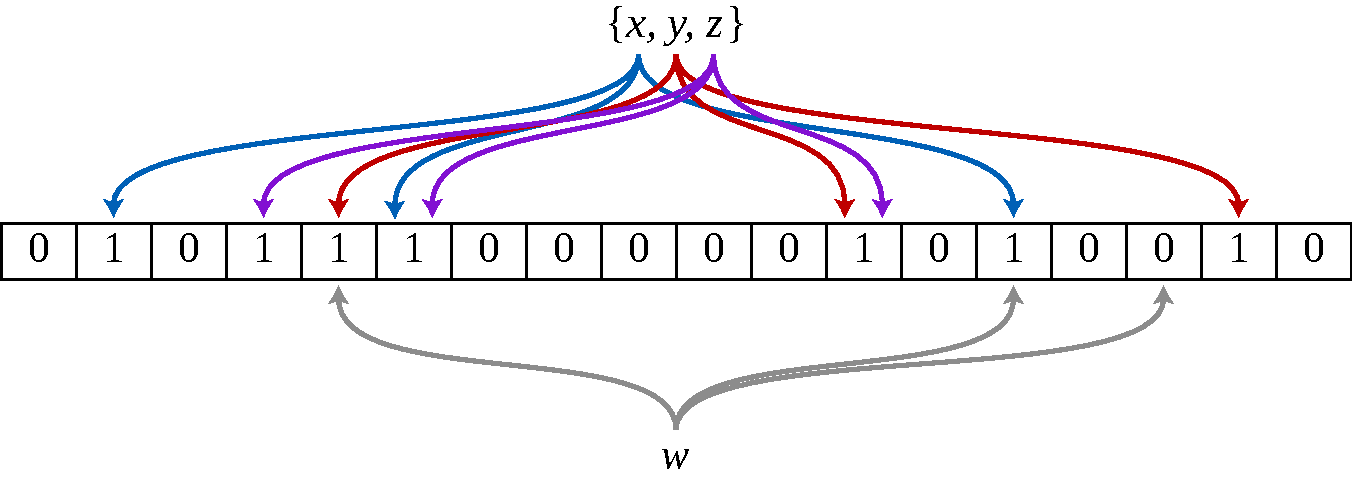
\includegraphics[width=\textwidth]{bloom-filter.pdf}
    \caption{Пример фильтра Блума с $m=18$ и $k=3$.}
\end{figure}

Фильтр Блума представляет собой битовый массив из $m$ бит. Изначально, когда структура данных хранит пустое множество, все $m$ бит обнулены. Пользователь должен определить $k$ независимых хеш-функций $h_i$, отображающих каждый элемент в одну из $m$ позиций битового массива достаточно равномерным образом.

Для добавления элемента $e$ необходимо записать единицы на каждую из позиций $h_i(e)$ битового массива.

Для проверки принадлежности элемента $e$ к множеству хранимых элементов, необходимо проверить состояние битов $h_i$. Если хотя бы один из них равен нулю, элемент не может принадлежать множеству (иначе бы при его добавлении все эти биты были установлены). Если все они равны единице, то структура данных сообщает, что $e$ принадлежит множеству. При этом может возникнуть две ситуации: либо элемент действительно принадлежит к множеству, либо все эти биты оказались установлены по случайности при добавлении других элементов, что и является источником ложных срабатываний в этой структуре данных.

Согласно \cite{broder02}, для заданных $n$~--- числа ожидаемых элементов в множестве и $p$~--- максимальной вероятности ложноположительного срабатывания возможно вычислить оптимальный размер $m$ как
\begin{equation}
    m=-\frac{n\ln p}{(\ln 2)^2},
\end{equation}
и оптимальное количество хеш-функций как
\begin{equation}
    k=\frac{m}{n}\ln 2.
\end{equation}

\subsection{Стандарт исключений для роботов} \label{ssec:robotstxt}
Следующая проблема, с которой нам предстоит столкнуться, заключается в том, что после получения новостной ленты нам необходимо сделать множество запросов к одному серверу, что обычно не нравится владельцам сайтов.

Когда владельцы сайта хотят ограничить доступ к определённым страницам для ботов, они используют для этого файл \verb|robots.txt|, находящийся в корне сайта (то есть по пути \verb|/robots.txt|). Это может быть полезно для ограничения частоты запросов со стороны роботов, запрета индексирования динамический и служебных страниц.

Формат файла имеет следующий вид:
\begin{verbatim}
<поле>:<необязательный пробел><значение><необязательный пробел>
\end{verbatim}

Стоит заметить, что вместо пробела могут использоваться также другие пробельные символы, а \verb|поле| является регистронезависимым.

Основные используемые поля:
\begin{itemize}
    \item \verb|user-agent|: стандартное поле, используется для задания имени бота, которому адресованы последующие правила, либо \verb|*|, если всем;
    \item \verb|disallow|: стандартное поле, используется для задания пути, индексация которого запрещена. В пути разрешены два спец-символа: \verb|*| (любое количество любых символов) и \verb|$| (конец пути). Причём путь, к примеру, \verb|/path/to/file| действует аналогично \verb|/path/to/file*|;
    \item \verb|crawl-delay|: нестандартное поле, используется для задания минимальной задержки в секундах между запросами со стороны робота.
\end{itemize}

\subsection{Разбор страницы}
Далеко не вся информация на странице ценна для поставленной задачи. Например, информация, размещённая в подвале и по сторонам страницы несёт обычно служебную информацию, которая может быть полезна при обходе страниц (так как может содержать полезные ссылки), но бесполезна конечному пользователю и не содержит информации, относящейся к новости. Поэтому ставится вопрос о выделении основного содержимого, то есть непосредственно текста новости, из html-страницы. Для этого необходимы методы выделения такой информации, которые в основном базируются на эвристики и неплохо работают во многих случаях \cite{pomikalek11}.

\subsubsection{Выделение основного содержимого} \label{sssec:readability}
Для получения основного содержимого во многих случаях достаточно сохранять только текстовые элементы HTML, то есть блоки текста, которые не прерывались разметкой, которые имеют более чем десяток слов. Люди выбирают один из двух типов текста для двух различных мотивов написания текста: <<навигационного>> и <<информационного>>.

Для элементов навигации обычно применяется текст, состоящий из нескольких слов (например, <<STOP>>, <<Прочтите это>>, <<Нажмите здесь>>), в то время как для основного содержимого используется много слов.

В то время как это разделение работает во множестве случаев, все становится сложнее с заголовками, короткими предложениями, отказами от ответственности, авторскими правами и другими колонтитулами.

Есть более сложные стратегии, а также функции, которые помогают отделять основное содержание от шаблонного \cite{kohlschutter10}:
\begin{enumerate}
    \item Рассмотренная выше плотность HTML-тегов;
    \item Ссылочная плотность (количество слов внутри ссылок по сравнению с общим количеством слов в блоке);
    \item Текстовые характеристики: количество запятых, длина текста и другие;
    \item Связь текущего блока с контекстом (с предыдущими и следующими блоками);
    \item DOM-структура документа (\verb|<article>|, \verb|<section>| и другие);
    \item Визуальное изображение страницы (например, большие изображения, окружённые текстом);
\end{enumerate}

Результирующий алгоритм, используя комбинацию этих факторов, рекурсивно оценивает все узлы документа, находя наиболее похожие на основное содержимое.

\subsubsection{Декодирование мнемоник HTML} \label{sssec:html-mnemonics}
Мнемоника~--- это конструкция SGML, которая ссылается на символ из набора символов текстового файла. В HTML предопределено большое количество спецсимволов. Чтобы вставить определённый символ в разметку, нужно вставить определенную ссылку-мнемонику в HTML-структуру.

Мнемоника имеет вид \verb|&...;|. Так, например, буква <<q>> может представляться как \verb|&#113;|, а <<--->> как \verb|&mdash;|.

\subsubsection{URL нормализация} \label{sssec:url-normalization}
Различные URL могут указывать на одну и ту же страницу, но отличаться при этом незначительно.

URL нормализация~--- процесс приведения URL к каноничному виду, путём применения различных правил трансляции адресов. Не все правила дают строго эквивалентные URL, однако на практике эти эвристики работают неплохо \cite{pant04}.

Ключ страницы~--- своего рода хеш, получаемый в результате агрессивной нормализации, то есть применения всех правил, указанных в данном разделе.

Ключ страницы может служит идентификатором новости, ленты и источника.

Относительно безопасные преобразования:
\begin{enumerate}
    \item Конвертация в нижний регистр компонентов схемы и хоста: \\ \verb|HTTP://www.Example.com/| в \verb|http://www.example.com/|;
    \item Удаление относительных каталогов, сегментов-точек: \\ \verb|http://example.com/../a/b/../c/./d| в \verb|http://example.com/a/c/d|;
    \item Удаление фрагментов: \\ \verb|http://example.com/bar.html#section1| в \verb|http://example.com/bar.html|;
    \item Удаление конечного слеша: \\ \verb|http://example.com/foo/| в \verb|https://example.com/foo|;
    \item Удаление порта по умолчанию: 80 для http и 443 для https \\ \verb|http://example.com:80| в \verb|http://example.com|;
    \item Перевод IDN в unicode: \\ \verb|http://xn--e1afmkfd.xn--80akhbyknj4f/| в \verb|http://пример.испытание/|.
\end{enumerate}

Преобразования, которые можно использовать для проверки эквивалентности двух страниц, но не при запросе:
\begin{enumerate}
    \item Удаление головного индекса (\verb|index.html|, \verb|default.aspx| и другие): \\ \verb|http://example.com/index.html| в \verb|http://www.example.com/|;
    \item Удаление дублированных слешей: \\ \verb|http://example.com/foo//bar.html| в \verb|http://example.com/foo/bar.html|;
    \item Удаление \verb|www.|: \\ \verb|http://www.example.com/| в \verb|http://example.com/|;
    \item Сокращение идентификаторов протокола: \\ \verb|https://example.com| в \verb|http://example.com|;
    \item Конвертация в нижний регистр всего URL: \\ \verb|HTTP://example.COM/TEST.html| в \verb|http://example.com/test.html|;
\end{enumerate}

Такие преобразование применимы для построения ключа страницы, но не для упрощения адреса ссылки.
